

% - What distillation is, and the four axes that organize it: signal, data source, timing, and teacher identity
% - White-box vs black-box: distilling from open weights vs strings
% - Off-policy distillation: generate from the teacher, then SFT on the outputs
% - On-policy distillation: sample from the student, score with the teacher in the loop
% - Distillation as reinforcement learning: the KD distance as a dense, token-level reward
% - Self-distillation: the model as its own teacher, and when that beats a stronger one
% https://github.com/burtenshaw/training-agents

\chapter[*合成数据生成]{*用于训练智能体式大语言模型的合成数据生成}\label{chap:synthetic-data}

%\chapter{*Synthetic Data Generation for Training Agentic LLMs}\label{chap:synthetic-data}

\begin{learningbox}
本章你将了解合成数据在智能体式大语言模型开发中所能扮演的角色。
具体而言，你将能够：
\begin{itemize}[leftmargin=*, nosep]
    \item 描述{\em 数据}在大语言模型训练流程中的重要性。
    \item 解释从更强模型向较弱学生模型{\em 蒸馏知识}的一般循环。
    \item 说明那些正在用合成数据替代人类生成内容的{\em 流程组件}。
    \item 概述{\em 筛选与评估}合成数据的各种策略。
    \item 通过描述使用人工生成数据的{\em 风险}，对比使用合成数据的优势与劣势。
\end{itemize}
\end{learningbox}

\section{数据的重要性}
大语言模型的快速规模化带来了对训练与评估数据的巨大需求。有人把训练数据称为{\em 数字石油}，以体现其作为人工智能发展首要原料的重要性。此外，数据正日益成为差异化因素，因为流程中的其他组件（例如模型架构）正在趋同 \citep{11072851}。随着模型持续规模化，它们需要从互联网抓取的数万亿词的人类生成文本；然而可用的人类生成数据是有限的，这就引出了训练数据是否会成为规模化主要瓶颈的问题，见图~\ref{fig:data-stock} \citep{villalobos2024position}。而且，随着数据需求规模增长，数据的获取在成本与时间上越来越难承受，因为大多数容易获取的来源正在枯竭。再者，隐私、版权与偏差等问题促使该领域把目光投向网页人类生成数据之外的途径，转而求诸合成数据生成 \citep{liang2022advances}。

\begin{figure}[tb]
    \centering
    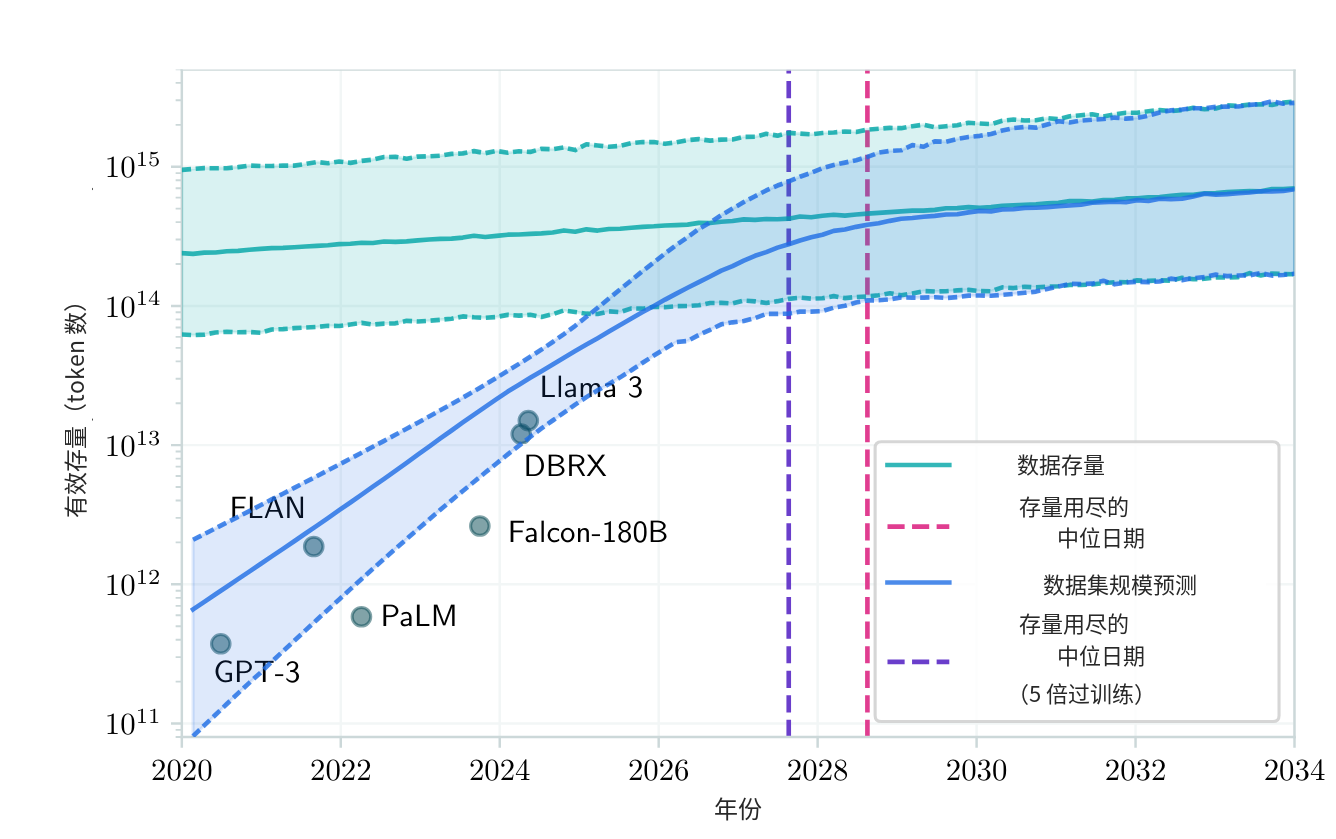
\includegraphics[width=0.7\linewidth]{part6/visuals/data_stock.png}
    \caption{用于训练大语言模型的可用人类生成公开文本与数据集规模的预测 \citep{villalobos2024position}。存量与数据集规模两条预测线的交点，标出了预计存量被完全用尽的中位年份（2028 年）。}
    \label{fig:data-stock}
\end{figure}

大语言模型正越来越多地生成用于训练下一代大语言模型自身的数据：模型被提示生成指令、对话、推理轨迹，乃至整份训练语料，再用这些内容去微调、蒸馏和评估其他模型 \citep{long-etal-2024-llms}。与采集并标注人类生成文本相比，这一自我强化循环降低了数据收集的成本与工作量，同时也对结果数据集的风格、难度与覆盖范围提供了细粒度控制。时至今日，这一做法已引起显著的工业界 \citep{10.1145/3715275.3732005} 与学术界 \citep{viswanathan-etal-2025-synthetic, alismail2025survey} 关注，其应用范围从通用指令微调，一直延伸到训练智能体行为（如工具使用、规划与多步推理）所需的更专门的数据（见第 \pageref{fig:virtuous} 页的图~\ref{fig:virtuous}）。

对模型生成数据的日益依赖，也在缩放定律（第~\ref{chap:scaling} 章）中引入了一个新术语，用来计入预训练语料中合成数据的比例。SYNTHLLM \citep{qin2025scaling} 等近期工作说明了这为何重要：它通过自动从源文档中抽取高层概念，并用基于图的算法重新组合，生成足够多样的合成语料，从而在各类模型规模上都遵循一条可预测的校正缩放定律。在这个版本的缩放定律中，收益更早开始趋缓（早于预训练中常用的其他 token 预算），而更大的模型在相对更少的 token 上就达到了最优性能。这表明合成数据不仅可以按体量调优，还可以按其产生的缩放曲线形状调优。

除缩放行为之外，为智能体能力——工具使用、规划与多步推理——生成数据，正越来越依赖协同的多智能体工作流，而非单一生成器模型。专门的智能体可以承担不同角色（例如提出任务、执行任务、评审结果），这往往能产生质量更高、更多样、结构上更贴近智能体训练实际所需的数据。Matrix \citep{wang2025matrixpeertopeermultiagentsynthetic} 是这一方向的一个例子：一个去中心化框架，其中控制流与数据流都被表示为智能体之间通过分布式队列传递的消息，使流程可以横向扩展而无需中央协调者。让我们更仔细地看一下合成训练流程。


\section{蒸馏循环}
\label{sec:distillation}
在智能体式大语言模型训练流程中使用合成数据，遵循的是整体蒸馏循环，如图~\ref{fig:synth-pipeline} 所示。一个生成器（一个强模型，或若干智能体的编排）用少量种子数据或真实数据生成一大池原始合成数据。该数据池随后经过\emph{筛选}（第~\ref{sec:data-cur} 节），再用于训练或\emph{蒸馏}一个模型。关键在于，所得模型本身可以成为下一轮迭代的生成器。这种自我强化循环的闭合，给训练稳定性与下游性能带来了相当大的风险（另见元学习中关于稳定性的讨论，第~\ref{chap:meta} 章）。

\begin{figure}[tb]
    \centering
    \resizebox{\linewidth}{!}{%
    \begin{tikzpicture}[
        node distance=7mm,
        box/.style={draw, rounded corners=2pt, align=center, minimum height=13mm, minimum width=23mm, font=\small, thick},
        data/.style={box, fill=blue!8},
        proc/.style={box, fill=orange!12},
        model/.style={box, fill=yellow!14},
        arr/.style={-{Stealth[length=2.5mm]}, thick},
    ]
        \node[data] (seed) {种子 /\\ 真实数据};
        \node[proc, right=of seed] (gen) {生成器\\[-1pt]{\scriptsize 教师 / 多智能体}};
        \node[data, right=of gen] (raw) {原始合成\\ 数据};
        \node[proc, below=9mm of raw] (inst-eval) {（内在）\\ 评估};
        \node[proc, right=of raw] (cur) {数据整理\\[-1pt]{\scriptsize 过滤、打分、去重}};
        \node[proc, right=of cur] (train) {训练 /\\ 蒸馏};
        \node[model, right=of train] (model) {模型\\ （学生）};
        \node[proc, below=9mm of model] (eval) {（外在）\\ 评估};
        \foreach \a/\b in {seed/gen, gen/raw, raw/cur, cur/train, train/model}
            \draw[arr] (\a) -- (\b);
        \draw[arr] (model) -- (eval);
        \draw[arr] (raw) -- (inst-eval);
        \draw[arr, dashed] (model.north) -- ++(0,6mm) -| (gen.north)
            node[pos=0.25, above, font=\scriptsize] {改进后的模型成为下一代教师};
    \end{tikzpicture}%
    }
    \caption{组织本章的合成数据循环。生成器由一小批种子数据产出原始合成数据，随后经筛选进行过滤与打分。数据训练或蒸馏出一个模型，该模型再被评估，并可用作下一轮迭代的生成器（虚线）。}
    \label{fig:synth-pipeline}
\end{figure}
蒸馏是合成数据生成的一个特例，其中生成器是一个\emph{我们试图迁移其能力的更强模型}。在知识蒸馏中，一个紧凑的\emph{学生}模型学习复制能力更强的\emph{教师} \citep{hinton2015distilling, hu2022teacherstudentarchitectureknowledgelearning}。它可以直接针对教师的输出预测做优化，也可以简单地用教师产出的合成数据来训练。蒸馏的目标是在推理时与数据成本两方面都得到一个更高效的教师版本，同时不过多牺牲任务性能。蒸馏已被广泛应用，包括在智能体场景中 \citep[e.g.,][]{li2025chainofagentsendtoendagentfoundation, du-etal-2025-agentic}。蒸馏也可用于为指令微调导出偏好数据。例如 Zephyr \citep{tunstall2024zephyr} 就是用 AI 反馈训练的：输出由强教师模型生成并排序，从而以极小的数据与训练成本使小模型对齐用户意图。

\paragraph{蒸馏的四个维度}
具体的蒸馏方法可以沿四个维度来组织。
%\begin{enumerate*}[label=(\number*)]
%\item 
(1) \emph{信号}：学生是模仿教师的 logits、完整的输出序列，还是由教师导出的标量奖励。
%\item 
(2) \emph{数据来源}：被评分的序列是由教师生成的，还是从学生采样的。
%\item 
(3) \emph{时机}：这些数据是一次性预先产生的（离策略），还是随着学生变化而持续产生的（在策略）。
%\item 
(4) \emph{教师身份}：教师是一个更强的独立模型，还是学生自身。
%\end{enumerate*}

下面我们逐一讨论蒸馏的这四个维度。
%already covered the first axis, the signal, in the discussion of soft targets, sequences, and rewards above; the following subsections outline the remaining three.

\subsection{信号：蒸馏目标}
当我们对教师的概率（$q$）拥有\emph{白盒}访问权时，学生 $p_\theta$ 被训练成使其下一 token 分布与教师一致。在蒸馏中，我们常用一个共享温度 $\tau$ 来软化分布（于是对 logits $z$ 有 $q^{\tau}(\cdot) \propto \exp(z/\tau)$）。在一个序列语料上的通用蒸馏损失为

% This is forward KL
\begin{equation}
    \mathcal{L}(\theta) = \mathrm{E}_{x}\left[ \sum_{t} D\big( q^{\tau}(\cdot \mid x_{<t}) \,\|\, p^{\tau}_\theta(\cdot \mid x_{<t}) \big) \right],
    \label{eq:kd}
\end{equation}
其中求和遍历 token 位置 $t$，$D$ 是一个散度（最常见的是 KL 散度），温度 $\tau > 1$ 会同时压平两个分布，使学生也能从教师的\emph{相对}置信度中学习。当只有教师的\emph{文本}可用时（\emph{黑盒}蒸馏，在从专有 API 蒸馏时是常见情形），我们不再能观察到 $q$，只能得到从它采样出的若干 token。软目标 $q^{\tau}(\cdot \mid x_{<t})$ 随之退化为采样 token 上的 one-hot 向量，散度 $D$ 变成 token 级交叉熵，式~\ref{eq:kd} 也就化为对教师生成结果的普通监督微调。在第~\ref{sec:sim-hum} 节我们将讨论 Self-Instruct 技术 \citep{wang-etal-2023-self-instruct}。这类方法从数据一侧进行蒸馏，因此属于黑盒方法。


\subsection{数据来源：教师—学生范式}
在蒸馏中，直觉上的假设是：更大更强的教师总是更好。然而存在例外 \citep{xu-etal-2025-stronger, li-etal-2025-small-models}。一个能力强的教师可能产出过长、过于复杂或风格不匹配的轨迹，小模型学生无法吸收。这一现象被称为\emph{小模型可学习性差距}。图~\ref{fig:small-model-learnability} 展示的情形是：小模型学生从较弱教师较短的推理中学到的，比从前沿模型繁复的思维链中学到的更多。其实际含义是，教师应当相对于学生当前的能力来选择，而不是孤立地追求最大化 \citep{zhang-etal-2026-find}。

\begin{figure}[tb]
    \centering
    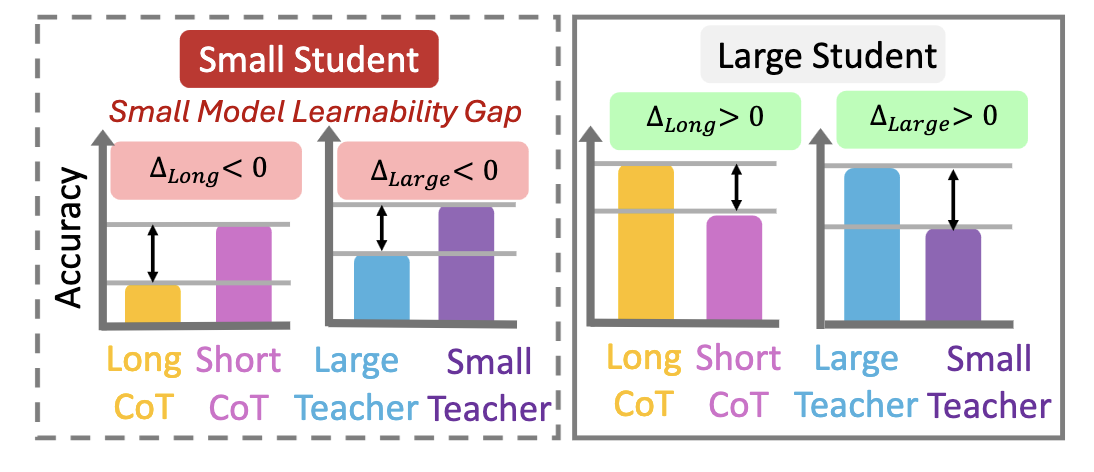
\includegraphics[width=0.8\linewidth]{part6/visuals/student_learner.png}
    \caption{小模型可学习性差距的可视化：小模型学生并不能始终从长思维链推理中获益，反而在用较小教师的较短思维链推理微调时表现更好 \citep{li-etal-2025-small-models}}
    \label{fig:small-model-learnability}
\end{figure}

\subsection{时机：离策略与在策略蒸馏}
第三个维度关乎时机。蒸馏中最常见的配方是\emph{离策略}蒸馏。这里我们从教师采样一个固定的补全数据集，再在其上微调学生（如上文黑盒情形）。这是一种简单且可并行的做法，但存在训练/推理不匹配：训练时学生只被展示过一次教师生成的 token 序列，而在部署时必须延续它\emph{自己}的、可能有缺陷的序列，这些序列可能与训练时见过的不同。这种{\em 暴露偏差}在长智能体轨迹上会不断累积。

\emph{在策略}蒸馏通过在循环内从学生自身采样序列、再由教师为其打分来解决这一问题。广义知识蒸馏（GKD）用教师对这些自生成序列的反馈来训练学生 \citep{agarwal2024policy}。学生恰好在它实际访问到的状态分布上被纠正。

这一在策略视角，使蒸馏通过模仿学习与强化学习之间的关联变得明确。式~\ref{eq:kd} 中逐 token 的教师散度充当一个\emph{稠密的、token 级奖励}。
蒸馏由此转化为一种强化学习形式：提供奖励信号的是教师，而不是稀疏的结果检查器 \citep{lu2025onpolicydistillation}。混合方案把这一思路推得更远：在强化学习阶段只在有益处选择性地模仿教师 \citep{zhang2026reinforcementaware}。

\subsection{教师身份：自蒸馏与自我改进}
教师模型与学生模型不必不同。当二者相同时，蒸馏就变成自我改进：模型生成候选解，保留通过检查的那些，并在其上训练。STaR \citep{zelikman2022star} 正是以这种方式自举推理能力：迭代地生成推理过程，保留那些能得到正确答案的，并在其上微调。

另一种方法是自我对弈微调（SPIN）\citep{chen2024self}。该方法让模型在多次迭代中区分自身生成与参考数据，从而在没有任何外部教师的情况下改进对齐。或许令人意外的是，即便\emph{重复}进行自蒸馏、不引入新数据源，也能带来可测量的收益——但只到某个限度为止 \citep{pareek2024understandinggainsrepeatedselfdistillation}。

当候选输出可以被廉价地\emph{验证}时，自我改进最为有力。在这种情况下，外部信号仍可被有效纳入。代码与数学中定义的问题就属于此类，因为解容易执行和检查。例如 CURE 是一个强化学习框架，其奖励从交互结果中共同演化模型的编码能力与单元测试生成能力。这里没有作为监督的真值代码。由于代码易于执行与检查，编码者与测试编写者充当相互适应的智能体，从而能够在困难问题上进行长程优化。同样的原理也支撑着自我挑战与自我演化的智能体：它们自己提出越来越难的任务，并随时间更新其生成策略 \citep{NEURIPS2025_a5a305fa, huang2025r, NEURIPS2025_d38653cd}。
\section{模拟人类生成的内容}
\label{sec:sim-hum}
从直接获取或从网页抓取的自然产生的人类生成文本转向别处，这一点或许最好从「精心整理的人类生成指令数据」向「合成生成扮演更核心角色的数据集」的演变中看出。下面我们讨论这些方法——它们的数据集在核心上仍以人类生成数据为基础。

作为人类仍支撑大部分数据的资源示例，Natural Instructions \citep{mishra-etal-2022-cross} 包含 61 个不同任务、由人类撰写的任务说明，以及 19.3 万个任务实例（输入—输出对）。这些说明采集自既有 NLP 数据集的说明文档，并统一映射到一个模式。对大语言模型的实验表明，模型在观察示例的同时观察说明会有所获益，尽管这些模型仍远低于估计的性能上界。

后续工作分别着眼于增加唯一任务与任务类型的数量 \citep{wang-etal-2022-super}、改变说明长度 \citep{bach-etal-2022-promptsource}，或纳入特别困难的任务 \citep{srivastava2023beyond}。重要的是，所有这些元数据集（数据集的数据集）最终仍建立于人类基准之上：其中每一个样本都由人撰写。因此，这类数据能自由地在网上找到多少，存在实际限制。

由于这些方法依赖以众包数据集形式存在的大量人工监督，近期工作转向生成扮演同一角色的合成数据。这里出现了 Unnatural Instructions \citep{honovich-etal-2023-unnatural} 等数据集，其中包含以极少人力收集的、富有创意且多样的指令，转而依赖对各类大语言模型的提示。实验表明，在略带噪声的 Unnatural Instructions 数据集上训练的模型，其结果与在高质量、人工整理的数据上训练相当，如图~\ref{fig:unnatural} 所示。这一结果表明，机器生成数据为扩充与多样化训练数据集提供了一个相对人力而言成本高效的替代方案。

\begin{figure}[tb]
    \centering
    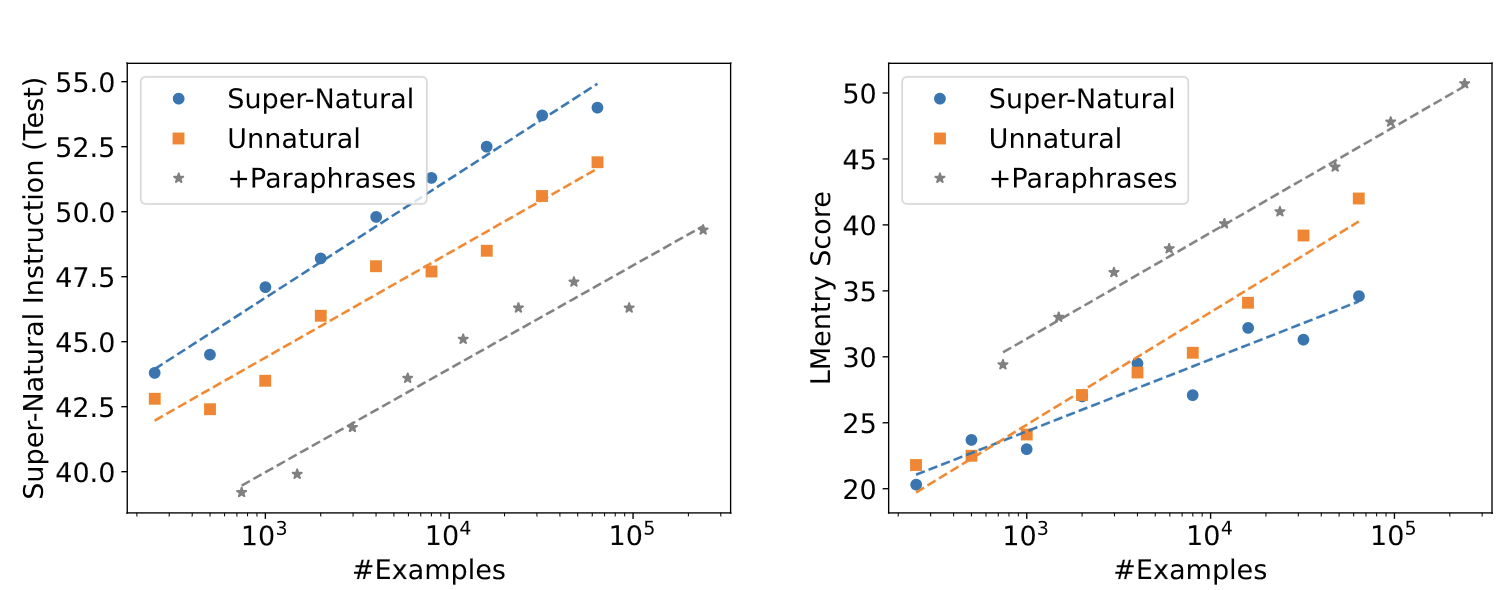
\includegraphics[width=0.8\linewidth]{part6/visuals/unnatural.png}
    \caption{将 Unnatural Instructions 与 Super-Natural Instructions 进行比较的缩放实验 \citep{honovich-etal-2023-unnatural}，在控制数据集规模的前提下考察模型性能，并在两个基准上测试：Super-Natural Instructions（左）与 LMentry（右）。}
    \label{fig:unnatural}
\end{figure}

由生成模型对人类式文本、代码与推理的模拟，为机器学习系统的训练与评估都开辟了新方法。通过提示强模型，研究者可以生成高度多样且复杂的数据集，以模拟人类的内容生成。例如 PersonaHub \citep{ge2025scalingsyntheticdatacreation} 用大规模人格集合来引导生成过程，借这些人格把大语言模型推向远比无条件下生成更多样的合成数据。

与自我改进类似，在输出相对易于验证的领域，用合成数据训练已显示出很大前景，例如数学 \citep{NEURIPS2023_44414694, liu2023tinygsmachieving80gsm8k}、编程 \citep{haluptzok2023language} 与游戏 \citep{wang2023voyager}。


\subsection{生成训练数据}
下面我们聚焦于生成训练数据。合成数据用于训练，已从一种小众的数据增强技术，转变为现代模型对齐与推理流程的核心组件。Self-Instruct \citep{wang-etal-2023-self-instruct} 等技术表明，较小的开放权重模型可以用完全由更强的专有模型生成的数据进行指令微调。该过程如图~\ref{fig:self-instruct} 所示：用一小批人工撰写的指令作为种子提示大语言模型，让它迭代地生成新的任务描述、输入与输出。这种模拟的人类内容使模型无需大批人工标注者即可获得复杂的零样本能力。
\begin{figure}[tb]
    \centering
    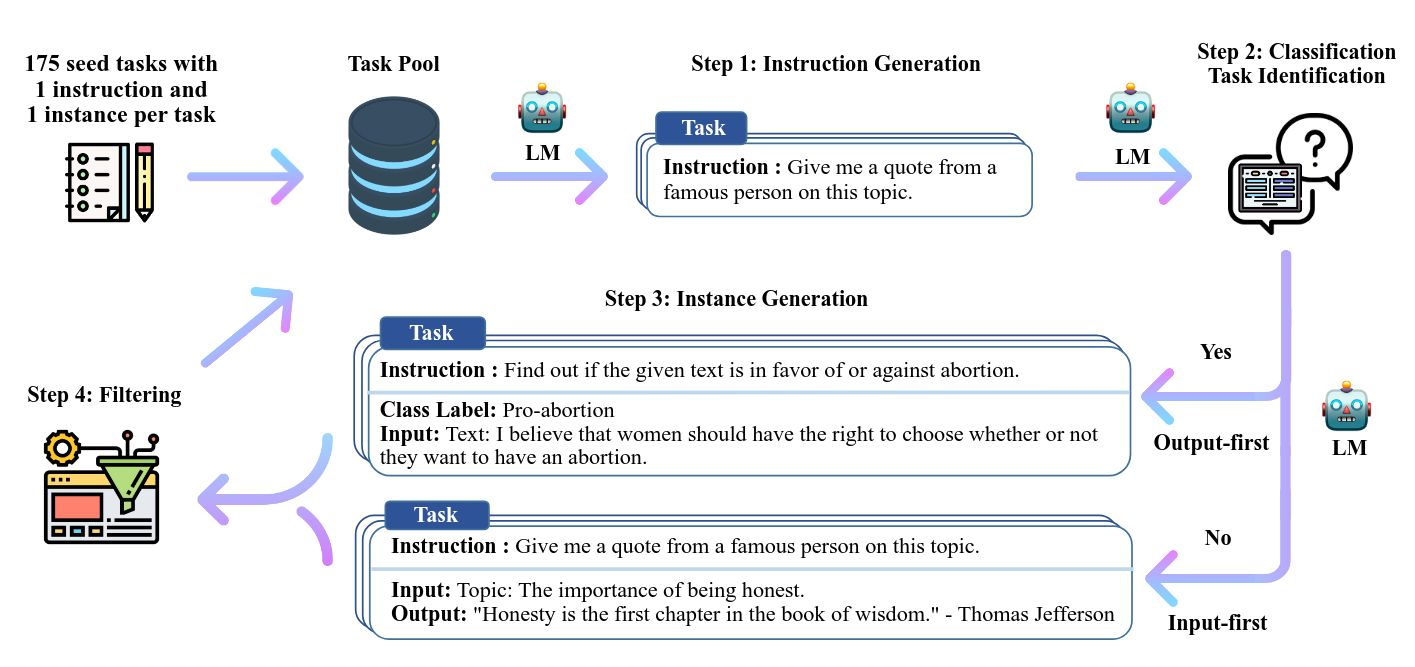
\includegraphics[width=\linewidth]{part6/visuals/self-instruct.png}
    \caption{Self-Instruct 流程 \citep{wang-etal-2023-self-instruct}。}
    \label{fig:self-instruct}
\end{figure}

\paragraph{利用既有数据}
另一些方法把精心整理的人类数据与合成数据结合，而不是以一种替代另一种。\citet{gunasekar2023textbooksneed} 表明，在人工撰写的教科书与合成生成文本的混合数据上训练，能产生能力很强的语言模型，这说明精心整理的人类数据与机器生成数据是互补而非替代关系。一个挑战是，合成生成的数据往往缺乏多样性，并会继承错误与幻觉，即便以人类生成数据作为种子也是如此。后续改进采用基于真值文档的生成过程 \citep{lupidi2025sourcesynth, NEURIPS2024_a4ca07aa}。
%, remedy these problems to a degree.


放大有限种子集的另一种互补方式是\emph{回译}。该方法最初引入于机器翻译，用来合成平行数据：把句子从源语言译到目标语言，再译回源语言 \citep{edunov-etal-2018-understanding}。同样的原理可以挪用到推理任务上：我们不再只为单个问题生成特定解，而是生成与既有解相容的新问题。MathGenie \citep{lu-etal-2024-mathgenie} 把这一想法用于数学推理：取一批种子「问题—解」对，先对解做增广，再把它们回译成新问题。由于每个新生成的问题都锚定在一个已验证的解上，这种做法既扩大了训练数据的规模与多样性，又减少了错误与幻觉。

\paragraph{人在回路方法}
全自动的生成流程并不总是够用。模型可能难以生成特定场景或领域相关的案例。这类失败的原因通常是生成用的大语言模型存在特定的盲点，这也使得生成真正有信息量的数据变得困难 \citep{lippmann2024illuminatingblindspotslanguage}。

此类问题促成了人在回路方法：由人来引导、过滤或修改机器生成的内容，而不是从头撰写。

WANLI \citep{liu-etal-2022-wanli} 把一个提出有挑战性自然语言推理示例的语言模型，与负责过滤和重标注的人类标注者配对，从而把自动生成的可扩展性与人类的质量控制结合起来。

EvalAssist \citep{santillan-cooper-etal-2025-synthetic} 把类似原理用于评估工具，用合成数据来支撑并加速人的判断。一种相关策略是让语言模型先产出初版种子文本，由人类评分者编辑后，再把结果用于自举一个更大的全合成数据集。这样一来，人力就花在纠正模型上，而不是撰写每一个示例。



\subsection{生成评估数据}
除训练之外，合成生成在评估中也扮演关键角色。传统静态基准面临快速的数据污染问题：测试集会不经意地泄漏进现代大语言模型的预训练语料。为缓解这一点，动态评估框架 \citep{kiela-etal-2021-dynabench} 日益依赖合成数据生成来创建定制的、一次性使用的测试用例。

此外，{\em 大语言模型作为评判者}范式 \citep{zheng2024judging} 通过提示一个强模型为其他模型的输出打分来模拟人类评估，使模型评分与人类偏好高度相关，并显著降低评估周期的延迟。

进一步构建专门的大语言模型难题基准，同样可以借助人在回路方法，例如 MATH$^2$ 基准。该基准用多个大语言模型通过多轮提示迭代生成并调整数学问题与解答，再由人类标注者扩充问题、检查答案，过程中同样有大语言模型辅助 \citep{shah2024ai}。高效生成合成评估数据的其他方法，则把标注者的任务从「想出新的样本」转变为「把样本改得更难」以应对大语言模型 \citep{yuan2021synthbio}。

\paragraph{自动化红队测试}
机器生成评估的一个具体用例，是借助\emph{自动化红队测试}进行面向安全的评估。在这一做法中，一个大语言模型生成对抗性提示，在部署前探测目标模型的漏洞 \citep{ganguli2022redteaminglanguagemodels}。通过合成大量潜在的恶意提示，研究者能够以人类红队无法企及的规模对模型做压力测试，使其对有毒输出、越狱与错位更具鲁棒性 \citep{perez-etal-2022-red}。由于同一批生成的提示随后还可用于针对这些失败对目标模型做微调，红队测试正好处在合成评估与合成训练数据的交界处。


\subsection{生成智能体数据}
在智能体场景中，数据必须针对整条轨迹来合成（而不只是单条指令—回答对）。当智能体与环境交互时，会产生一整套工具调用、观察与决策的序列 \citep{kang2025distilling}。这超出了训练或评估一个处理单个输入—输出对的普通大语言模型所需的数据。尽管通常仍用同样的生成模型来产出，生成智能体数据比生成用于指导底层大语言模型本身的数据要复杂得多。让我们看一个例子。


\begin{example}
考虑为一个使用工具的智能体合成单条训练轨迹，大致沿用 APIGen-MT \citep{NEURIPS2025_5e3661f7} 的两阶段配方。

首先，一个\emph{任务提议者}发明一个看似合理的用户目标、一组可用工具，以及一个真值答案：

\emph{用户：}「这个周末莱顿的天气怎么样，我要不要带伞？」\quad \emph{工具：} \texttt{get\_forecast(city, days)}。

随后一个\emph{执行者}模型展开这段交互，先发出中间的工具调用、消费其（模拟的）观察结果，然后作答：

\begin{center}\small
\texttt{get\_forecast("Leiden", 2)} $\rightarrow$ \texttt{\{sat: rain, sun: clear\}} $\rightarrow$ \emph{``周六有雨，周日晴——周六请带伞。''}
\end{center}

最后，一个\emph{验证器}检查所发出的调用是否形式良好、其参数是否与请求匹配、最终答案是否与观察一致。只有通过验证的轨迹才会被保留。

请注意需要被合成的东西：不只是一对输入—输出，而是目标、工具模式、调用、观察，以及一个验证整条轨迹的检查器。
\end{example}
智能体数据的生成方法通常涉及整套智能体编排，以进行包含人类输入与工具使用的多轮对话 \citep{wu2024autogen}。APIGen-MT \citep{NEURIPS2025_5e3661f7} 以一个两阶段框架体现了这一转变，用于生成可验证且多样的多轮智能体数据。TOUCAN \citep{xu2025toucansynthesizing15mtoolagentic} 以更大规模追求类似目标，通过模拟真实的工具调用来构建大型工具—智能体数据集。除了为固定技能生成轨迹之外，一些工作显式地合成数据，以把一项新技能或行为从强模型迁移到较弱模型，这一过程被称为生成式教学 \citep{crispino2023agent}。此外，智能体合成数据并不限于文本，类似的生成流程也延伸到图像、表格数据以及其他形式的交互或行为数据。

对于智能体合成数据的生成，控制任务复杂度是一个反复出现的挑战。例如，深度研究型智能体旨在通过与在线工具的长程交互来解决复杂的问答任务，但通常用于训练它们的数据缺乏对难度与质量的细粒度控制，产生的合成数据不足以捕捉足够的复杂度。\citet{pandit2025synthesizingagenticdataweb} 用一个流程解决了这一问题：合成出的问答对会逐步提高任务复杂度，直到前沿基线网页智能体失败为止。这种课程学习式做法直接依据智能体能力来校准任务难度，而非依赖固定的启发式规则。

AReaL-SEA \citep{gao2026selfevolvingsyntheticdataverifiablereward} 从互补的角度处理可靠性问题。这里，一个多智能体引擎合成以工具为依据的对话，并配合可执行的逐实例检查器。随后，一个闭环的自我演化过程随时间更新提示，以提升可靠性。



\section{数据筛选}
\label{sec:data-cur}

合成数据生成之后，我们需要检查其质量并加以筛选。通常这意味着过滤、打分与挑选样本，只保留有用的示例。评估合成数据的有用性可以有两种互补方式：\emph{外在}方式，即度量其对下游任务的影响；或\emph{内在}方式，即直接考察生成数据（或生成过程）的性质。

在实践中，筛选被实现为一个多阶段过滤流程，把下文讨论的各项准则转化为具体的算子。典型阶段包括\emph{语义去重}（通过嵌入相似度移除近重复样本以保持多样性）、\emph{困惑度过滤}（用参考模型丢弃不连贯或分布外的文本）、基于规则或格式的检查，以及\emph{奖励模型或评判者打分}以只保留高保真样本。那篇开创性的{\em 教科书就是你所需要的一切}论文 \citep{gunasekar2023textbooksneed} 提醒我们：这一筛选步骤的重要性往往不亚于数据体量——为质量而做的激进过滤可以胜过纯粹的数量。缺少这一步，模型很容易学到教师的生成痕迹与统计异常。

\subsection{外在评估}
外在评估回答一个简单问题：合成数据对下游任务真的有帮助吗？这个话题也被称为\emph{效用}。实践中，效用通过在合成数据（单独或与真实数据混合）上训练或微调模型，再在一个留出的真实世界测试集上评估来衡量。外在评估是合成数据是否有用的最直接度量。例如，若纳入合成数据后预训练模型的性能（例如以困惑度衡量）提升，我们就可以断定该数据有用。然而它也是最昂贵的：在得到任何信号之前都需要一次完整训练。如果我们改动生成过程或选择另一个数据子集，就需要重新训练并评估模型。这使得外在评估不适合在生成过程中用于过滤或挑选单个示例。


\subsection{内在评估}
内在评估转而考察生成结果自身的特性，无需承担下游训练的成本。已有若干质量方面被提出用于评估合成文本 \citep{ramesh-etal-2025-synthtexteval}。除了在输出层面评估，也可以直接对生成过程所用语言模型做基准测试 \citep{kim-etal-2025-evaluating}。这能比检查生成数据更早、更廉价地给出信号。


\paragraph{数据正确性}
一个生成的示例只有在其内容在事实与逻辑上站得住脚时才有用。由于合成数据往往来自其他大语言模型，它会继承生成模型的失效模式，包括虚构的事实、不一致的推理，或与内容不匹配的标签。这些错误随后会传播进在其上训练的模型。正确性通常通过以下方式检查：把生成结果与人类生成的标签对比 \citep{long-etal-2024-llms, chim-etal-2025-evaluating}；执行验证（例如基于规则的检查器或单独的评判模型）\citep{chen-etal-2025-mastering, yang-etal-2025-longfaith, NEURIPS2024_4b77d5b8}；或对同一输入的多次生成做一致性检查 \citep{NEURIPS2022_639a9a17, seegmiller-etal-2025-flames}。


\paragraph{数据多样性}
创建合成数据的一个关键问题是保持多样性。logit 抑制与温度采样可以改善数据多样性，但要以数据正确性为代价 \citep{chung-etal-2023-increasing}。多样性也难以度量：词汇启发式（例如 ROUGE）或神经启发式（基于嵌入的相似度）常被用作代理，但各自只捕捉到数据中可能变异的一小部分。

MetaSynth 通过元提示生成能增强多样性的合成数据来解决这一问题：由一个语言模型编排多个专家大语言模型智能体，协同生成数据 \citep{riaz-etal-2025-metasynth}。


\paragraph{数据污染}
合成数据的一个严重风险是污染 \citep{deng-etal-2024-unveiling, balloccu-etal-2024-leak}。生成用的大语言模型是在大型、过滤不完善的网页数据集上预训练的，可能记住了基准，并在被提示生成新训练示例时复现或近似改写它们。
%This means, much like the case of downward spirals of decreasing data diversity, that 
经过多步之后，合成生成的数据会收敛到既有基准之上。这会人为抬高评估分数，例如在代码生成基准的情形中 \citep{matton-etal-2024-leakage}。针对这类泄漏的解决方案应超越简单的精确匹配过滤，需要对已知基准做 n-gram 重叠搜索、成员推断式探测 \citep{puerto-etal-2025-scaling, huang-etal-2026-robust}，或动态数据集构建流程 \citep{chen-etal-2025-benchmarking-large}。

\paragraph{公平性与偏差}
大语言模型会从自身训练数据中继承并放大社会偏差。如果我们反过来用这些大语言模型生成合成语料，就有进一步固化刻板联想、扭曲人口统计表征，或造成不同社会群体间生成质量不均的风险 \citep{gallegos2024bias}。这对合成数据尤为值得警惕，因为它是大规模产出的，且往往直接被当作新大语言模型的训练材料。

最后，内在指标只是有用性的代理。一个数据集可能在多样性上得分很高，或通过正确性检查，却未能改善甚至损害外在评估。词汇与神经多样性启发式度量的是表层变异，可能漏掉真正要紧的冗余（例如重复的推理模式），也可能高估多样性。% which is not useful for downstream tasks. 
正确性检查还依赖于存在可信的参照、基于规则的验证器或评判模型——而对于开放式或主观的生成，这些可能并不存在，或并不可靠。基于这些原因，内在评估最好被视为一项附加检查，而非外在评估的真正替代。




\section{风险}
\label{sec:risks}

读到这里应当已经清楚：用合成数据训练智能体式大语言模型，是一个并非没有问题的方案。我们还将讨论与合成数据相关的若干其他风险，包括模型崩塌、偏差放大、安全与隐私漏洞，以及法律与伦理方面的关切。

\subsection{模型崩塌}
图~\ref{fig:synth-pipeline} 中循环的定义性风险在于：它以自身输出为食。\emph{模型崩塌}是一种已有充分记载的现象：在递归生成的 AI 数据上训练一代又一代模型，会导致原始分布的多样性消失 \citep{shumailov2024curserecursiontraininggenerated}。稀有事件与低概率的语言细微差别被采样到的机会变少，于是每一代都会多遗忘一点分布的长尾行为，直到模型收敛为一个重复的、高概率的模型。一些实验表明，在纯合成数据上反复训练会带来递减、最终为负的回报 \citep{singh2024beyond}；而把语料集中于少数合成来源（而非多个来源），会加剧所得模型的脆弱性 \citep{schaffelder2025syntheticeggsbasketsimpact}。类似地，从教师蒸馏出的小模型学生容易产生幻觉，且常在长尾知识上失败 \citep{pmlr-v202-kandpal23a}。更微妙的是，模仿教师可能造就一个在\emph{风格}上贴近教师、却在\emph{事实性}上落后的学生，而这种差距通常只有通过有针对性的能力基准才会暴露 \citep{gudibande2023falsepromiseimitatingproprietary}。标准的缓解办法是持续用真实人类数据锚定语料，而不是仅靠合成数据训练。

\subsection{偏差放大}
由于生成模型过度表征其训练分布中的多数模式，合成数据往往会削去自然人类话语中多样的长尾视角 \citep{van-der-meer-etal-2024-empirical}。因此，在这种数据上训练出的学生可能表现出教师社会偏差的放大、漫画化版本。学生模型会复现刻板联想、扭曲的人口统计表征，或群体间不均的生成质量 \citep{gallegos2024bias}。这一关切对合成数据比对原始模型输出更大，因为数据是大规模产出的、直接被当作训练材料消费，且循环的每一轮都会叠加前一轮的影响。

\subsection{安全风险}
合成训练数据还带来安全风险。依赖生成数据为恶意污染训练数据引入了新的攻击面。如果教师模型或生成流程的任何环节被攻破，对手就能发动数据投毒攻击。由于合成语料通常大到无法彻底审计，细微的后门或恶意的指令—回答对可以被植入，并一直潜伏到在部署的学生模型中被触发。已有研究表明，即便只污染网页规模语料中极小的一部分，也是可行且廉价的 \citep{carlini2024poisoning}；而当「教师」是一个训练数据与对齐方式都不透明的、不受控的第三方模型时，风险会更高。

\subsection{隐私保护}
合成生成常被提及为数据隐私的解决方案。其想法是：合成数据不含个人可识别信息（PII）\citep{dwork2014algorithmic}，却能反映私有数据（如医疗记录）的统计性质。

然而，这类数据存在相当大的记忆风险。若在生成阶段没有严格的隐私保证，生成模型可能无意中重建、从而泄漏其最初训练所依据的敏感人类数据的确切片段 \citep{274574}。
隐私评估表明，现成的隐私保护方法可能失效 \citep{ramesh-etal-2024-evaluating}。

常见的隐私方法依赖差分隐私 \citep{dwork2006calibrating}：这是对生成过程的一种保证，界定了当数据集中加入或移除某个个体的记录时，输出分布最多能改变多少。这个界由一个隐私预算控制，取值越小保护越强，代价是效用损失越大 \citep{yue-etal-2023-synthetic}。


\subsection{版权与使用条款}
合成数据吸引力的一部分在于，它绕开了抓取互联网规模人类文本这一法律地位尚不明确的做法——后者已引发版权诉讼。%with unresolved international boundaries. 
2025 年美国 \emph{Bartz 诉 Anthropic} 案的和解颇具说明性。地区法院认定，大语言模型训练本身具有{\em 极高}的转换性，因而属于合理使用的候选；然而责任仍产生于底层语料的\emph{获取}方式，即摄入了数十万本盗版书籍，Anthropic 以每部作品约 \$3{,}000 达成和解（总额约 15 亿美元），其他案件（如 \emph{Kadrey 诉 Meta}）中也有类似情形。这表明，训练所依据的数据正日益受到版权与使用条款的审视。

合成数据并不能完全绕开这一问题。从专有模型蒸馏引出一个不同的问题：多数商用大语言模型 API 的服务条款明确禁止用其输出来训练竞争模型。因此，由黑盒教师生成的数据，无论版权如何，都可能在法律上有问题。这种张力在 2025 年公开浮现：有人指控竞争系统是在前沿 API 的输出上训练的。对实践者而言，这意味着\emph{生成器}的许可与其所替代的任何人类数据的许可同样重要，都需要核查。


\section{结语}
合成数据已从一种小众的增广方法，转变为大语言模型流程的核心成分（第~\ref{chap:pipeline} 章），其驱动力是人类文本将成为规模化瓶颈这一前景（第~\ref{chap:scaling} 章）。强模型与多智能体编排可以模拟指令数据、评估基准，以及更晚近的、由工具调用与决策构成的完整智能体\emph{轨迹}（第~\ref{chap:agents} 与~\ref{chap:tools} 章）。

由于原始生成结果带有噪声，筛选、外在效用，以及对正确性、多样性与污染的内在检查，与生成本身同样重要。各种设置都可以被视为知识蒸馏的不同形式，沿信号、数据来源、时机（离策略 vs.\ 在策略）与教师身份这四个维度组织。

把同一模型的合成数据复用于自我改进，有望实现可验证的推理（第~\ref{chap:reasoning} 章）。然而，在所有这些流程中，我们都需要留意这些模型在消费什么数据：缺少真实数据锚定与细致审计，模型崩塌、偏差放大、安全、隐私与许可风险都会随每次迭代而叠加。

\bibliographystyle{plainnat}
\bibliography{agenticbook,refs,case,synthetic}
